\documentclass[11pt,a4paper]{article}
\usepackage[top=3cm, bottom=3cm, left=2.5cm, right=2.2cm]{geometry} %geometry of page
\usepackage[hidelinks]{hyperref} %reference links
\usepackage{fancyhdr} %header and footer control
\usepackage{minted} %source code syntax highlighting
\usepackage{qrcode} %qrcode links
\usepackage{graphicx} %images
\usepackage{tikz}

\linespread{1.3}
\emergencystretch 3em

% Set Header and Footer
\fancyhead{}
\fancyhead[L]{\textbf{Lab 2: External LED}}
\fancyhead[R]{d.s.brennan@sheffield.ac.uk}
\fancyfoot{}
\fancyfoot[L]{\thepage}
\fancyfoot[R]{MAC 233 Arduino Labs, School of MAC, University of Sheffield}

% Create Document
\begin{document}
\pagestyle{fancy}

\section*{Prerequisites}
This worksheet builds upon the Lab 1 worksheet. You will have needed to complete the Lab 1 worksheet before you can continue with this lab. Out of your Arduino pack, you will need: 1 Arduino, 1 breadboard, 1 LED, 1 $220\Omega$ resister, and 1 jumper cable.

\section*{Objectives}
The objective of today's lab is to learn how to use an electronic breadboard to create a circuit and to control an external output on the Arduino.\\

\noindent
We will be taking the scenario from the previous worksheet and changing it to communicate with an external LED. Whilst this may sound complex, we are able to use the code from the previous worksheet as a starting point; therefore, it is only one new line of code and changing three existing lines of code.

\section*{Understanding a Breadboard}
An electronic breadboard is a useful tool to create quick circuits. It becomes particularly helpful in our use case, as we can place our Arduino within the breadboard without any further adapters.\\

\noindent
A breadboard can be thought of as a collection of rows (1\textrightarrow $N$) and columns (A\textrightarrow J). Each row is wired together into two groups --- divided by the centre separator. The first group is the columns A\textrightarrow E (in our example included in Figure \ref{fig:breadboard-groups}), and the second group is columns F\textrightarrow J. Each row is numbered from 1\textrightarrow $N$. Any item plugged into a pin will be accessible by any other pins within that pins row group.\\

\begin{figure}[ht!]
    \begin{center}
        \begin{tikzpicture}[
            highlight/.style={draw=purple, line width=.25mm},
        ]
            %%breadboard
            \node[] at (0, 0) {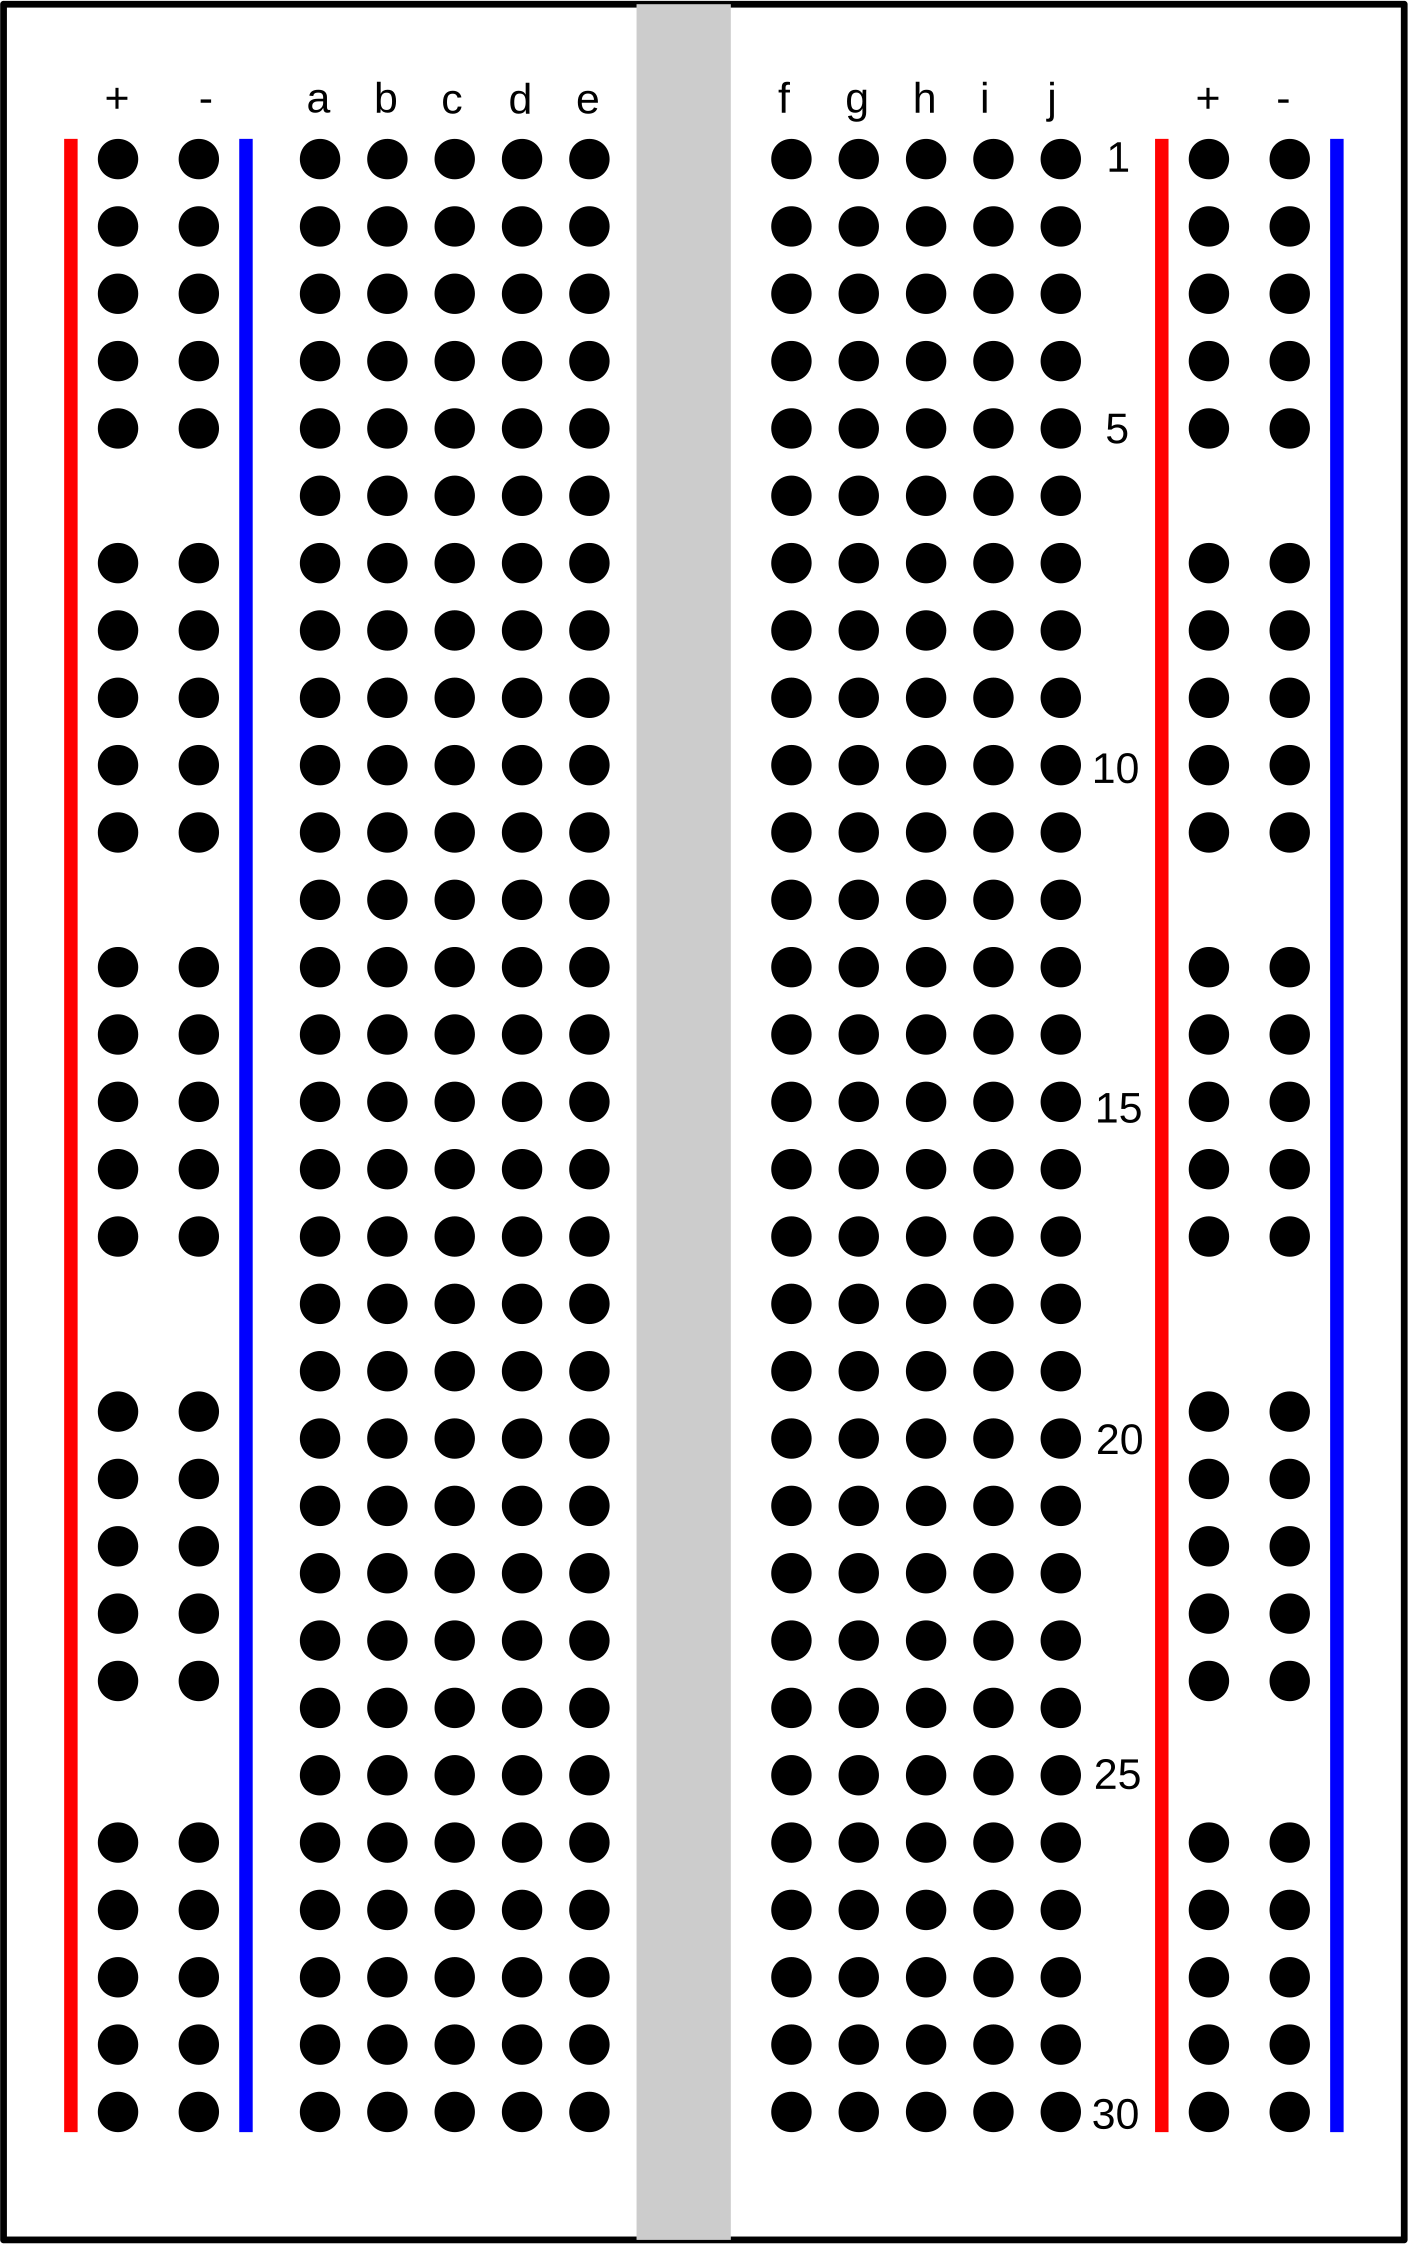
\includegraphics[width=.5\textwidth]{./images/breadboard.png}};
            %%areas
            \draw[highlight] (-2.36, 5.43) rectangle ++(1.86, 0.3);
            \draw[highlight] (0.36, 5.43) rectangle ++(1.86, 0.3);
            \draw[highlight] (-3.54, -5.9) rectangle ++(0.3, 11.65);
            \draw[highlight] (-3.07, -5.9) rectangle ++(0.3, 11.65);
        \end{tikzpicture}\\
        \scriptsize
        Original image source: \url{https://freesvg.org/breadboard}
    \end{center}
    \caption{An example electronic breadboard. There are four groups highlighted. The positive and negative column groups, and the two groups that are wired together for each row.}
    \label{fig:breadboard-groups}
\end{figure}

\noindent
For instance, if you plugged the Arduino output for Pin D2 into column H on row 13, you would then be able to plug in an LED leg into column J on row 13. This would create a complete circuit --- given that you have also completed the part of the circuit for the other LED leg.\\

\noindent
There is also four power rails at either side of the breadboard --- two on the left, and two on the right. The rails on either side are traditionally used for positive and negative power. In our case this would be used for +5v and GND. All the rows within a rails column are considered connected together. Figure \ref{fig:breadboard-groups} depicts the two power rail groups on the left side of the breadboard, as well as depicting the two row groups for row 1.

\section{Creating the circuit}
The circuit needed for this worksheet is: Arduino Pin D2 \textrightarrow $220\Omega$ resister \textrightarrow LED
\textrightarrow Arduino GND.\\

\noindent
To do this, place your Arduino into the breadboard. Once this is done, use the pin out diagram linked in lecture 1 to find which pin on the Arduino is Pin D2. You then need to connect one leg of the $220\Omega$ resister to Pin D2 of your Arduino through your breadboard. Then connect the other leg of the $220\Omega$ resister  --- mind how the rows and columns are connected, ensure the resister isn't bypassed in the circuit --- to the positive leg of the LED (the longer leg). Finally, connect the negative leg of the LED to the ground PIN on your Arduino through the jumper cable. You won't see anything visual happen at this stage, you need to complete the code tweaks below before the LED will light up.

\section{Changing the existing code}
Firstly, open your sketch from the previous worksheet into Arduino IDE. Once this is open, save the sketch under a new name (`File'\textrightarrow `Save As'). This will make sure you still have a copy of the sketch from Lab 1.\\

\noindent
The first thing we are going to do is create a new definition for a `$LED\_PIN$' which will map to the Arduino Pin D2. To do this, copy the code below at the top of your file (before the Morse code definitions).

\inputminted{arduino}{./src/1-pin-definition.txt}

\noindent
The internal LED on an Arduino is referenced in exactly the same way as you would reference an external pin. This means all we need to do is change anywhere within our code that uses `$LED\_BUILTIN$', to use the newly defined external pin `$LED\_PIN$'. This means changing the code to the following lines:

\inputminted{arduino}{./src/2-pins.txt}

\noindent
You now should be able to compile your sketch (`Sketch'\textrightarrow `Verify/Compile') and then upload to your Arduino (`Sketch'\textrightarrow `Upload'). You should see that your Arduino now blinks the externally connected LED in the same pattern as it did on your internal LED.

\section*{Help}
If you are having issue compiling the project or don't understand where each section goes, you can see a complete version of the sketch with additional source code comments at \url{https://github.com/dsbrennan/mac-233-arduino-labs/blob/main/lab-2-led/lab-2-led.ino}.

\vspace{2em}

\begin{center}
    \qrcode[hyperlink, height=4cm]{https://github.com/dsbrennan/mac-233-arduino-labs/blob/main/lab-2-led/lab-2-led.ino}
\end{center}


\end{document}